%!TEX program = xelatex
\documentclass{beamer}
%\usetheme{Boadilla}  
\title{Uio Driver Modification For AXI-Stream IP} 
\author{Liu,Yu-Tang}
\date{\today} 
\begin{document} 

\maketitle  % 封面

%p1
\begin{frame}
\frametitle{Outline}
\begin{itemize}
\item Embedded Linux on zedboard
\item UIO driver
\item DMA and AXI4
\item UIO driver modification
\end{itemize}
\end{frame}

%p12
\begin{frame}
%\frametitle{}
%\begin{itemize}
\centering Embedded Linux on zedboard
%\end{itemize}
\end{frame}






%p3. Embedded Linux on zedboard  @2
\begin{frame}
\frametitle{Embedded Linux on zedboard}
\begin{figure}
\centering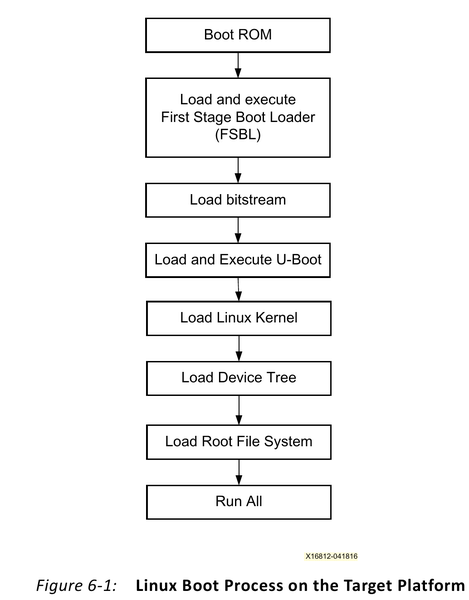
\includegraphics[scale=0.35]{boot.png}

\end{figure}
\end{frame}




%p2. Embedded Linux on zedboard  @1
\begin{frame}
\frametitle{Embedded Linux on zedboard}
\begin{itemize}
\item Phase 0
	\begin{itemize}
	\item Load boot rom
	\item Check JP7-JP11
	\end{itemize}
\item Phase 1
	\begin{itemize}
	\item FSBL
	\end{itemize}
\item Phase 2
	\begin{itemize}
	\item Software 
	\end{itemize}
\end{itemize}
\end{frame}


%p4
\begin{frame}
\frametitle{Embedded Linux on zedboard}
\begin{itemize}
\item So we need ....
	\begin{itemize}
	\item Boot.bin
	\item Uboot
	\item devicetree
	\item rootfs
	\end{itemize}
\end{itemize}
\end{frame}

%p5
\begin{frame}
\frametitle{Embedded Linux on zedboard}
\begin{itemize}
\item Boot.bin
	\begin{itemize}
	\item fsbl.elf
	\item boot.elf
	\item vivado-design.bit
	\end{itemize}
\end{itemize}
\end{frame}

%p6
\begin{frame}
\frametitle{Embedded Linux on zedboard}
\centering Uboot
\centering \\
\begin{itemize}
	\item Das U-Boot (subtitled "the Universal Boot Loader" and often shortened to U-Boot) is an open source, primary boot loader used in embedded devices to package the instructions to boot the device's operating system kernel.
\end{itemize}
\end{frame}


%p7
\begin{frame}
\frametitle{Embedded Linux on zedboard}
\begin{figure}
\centering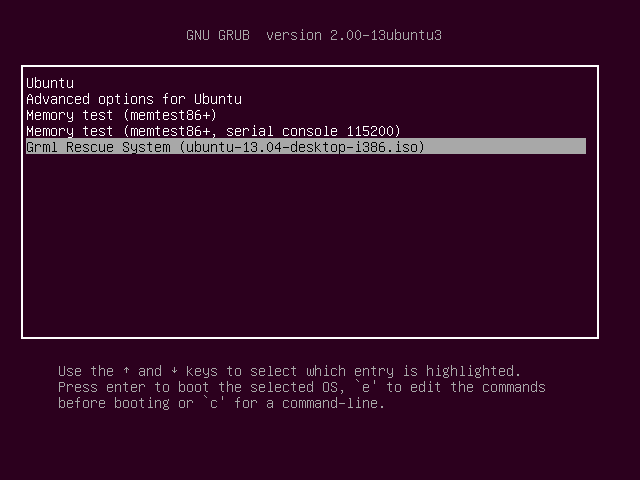
\includegraphics[scale=0.35]{grub.png}
\caption{grub}
\end{figure}
\end{frame}

%p8
\begin{frame}
\frametitle{Embedded Linux on zedboard}
\centering devicetree\\
\begin{itemize}
	\item In computing, a device tree (also written devicetree) is a data structure describing the hardware components of a particular computer so that the operating system's kernel can use and manage those components, including the CPU or CPUs, the memory, the buses and the peripherals.
\end{itemize}
\end{frame}

%p8
\begin{frame}[fragile]
\frametitle{Embedded Linux on zedboard}
\begin{figure}
\centering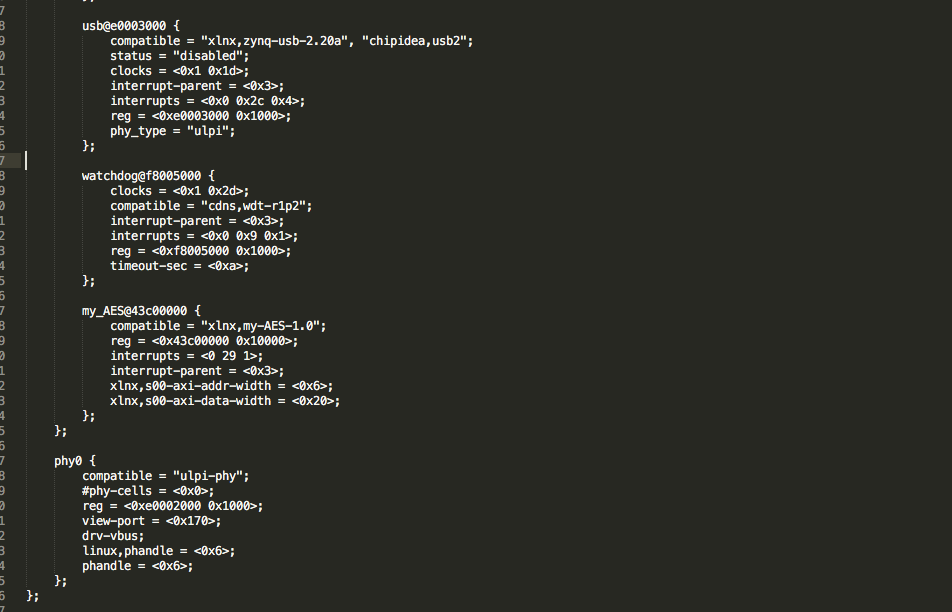
\includegraphics[scale=0.3]{devicetree.png}
\end{figure}
\end{frame}

%p9
\begin{frame}
\frametitle{Embedded Linux on zedboard}
\centering root file system
\centering \\
\begin{itemize}
	\item The root filesystem is the filesystem that is contained on the same partition on which the root directory is located, and it is the filesystem on which all the other filesystems are mounted (i.e., logically attached to the system) as the system is booted up (i.e., started up). 
\end{itemize}
\end{frame}


%p11
\begin{frame}
\frametitle{Embedded Linux on zedboard}
%\begin{itemize}
\centering Now we can run linux on zedboard!\\
%\end{itemize}
\end{frame}

%p12
\begin{frame}
%\frametitle{}
%\begin{itemize}
\centering UIO driver
%\end{itemize}
\end{frame}


%p13
\begin{frame}
\frametitle{Uio Driver}
\centering About UIO
\centering \\
\begin{itemize}
\item only one small kernel module to write and maintain.
\item develop the main part of your driver in user space, with all the tools and libraries you’re used to.
\item bugs in your driver won’t crash the kernel.
\item updates of your driver can take place without recompiling the kernel.
\end{itemize}
\end{frame}

%p14
\begin{frame}
\frametitle{Uio Driver}
\centering How UIO works?\\

\begin{itemize}
\item Each UIO device is accessed through a device file and several sysfs attribute files. 
      The device file will be called /dev/uio0 for the first device, and /dev/uio1, /dev/uio2 and so on for subsequent devices.

/dev/uioX is used to access the address space of the card. Just use mmap() to access registers or RAM locations of your card.


\end{itemize}
\end{frame}




%p15
\begin{frame}[fragile]
\frametitle{Uio Driver}
\centering How to use UIO\\
\begin{verbatim}
int fd = open("/dev/uio0", O_RDWR);

void *ptr = mmap(0, 0x10000, PROT_READ|PROT_WRITE, MAP_SHARED, fd, 0);

volatile uint32_t *ctrl = (uint32_t *)ptr;
volatile uint32_t *memA = (uint32_t *)ptr + 1;
\end{verbatim}
\end{frame}



%p20 兩個design 圖比較
\begin{frame}[fragile]
\frametitle{Uio Driver}
\begin{figure}
\centering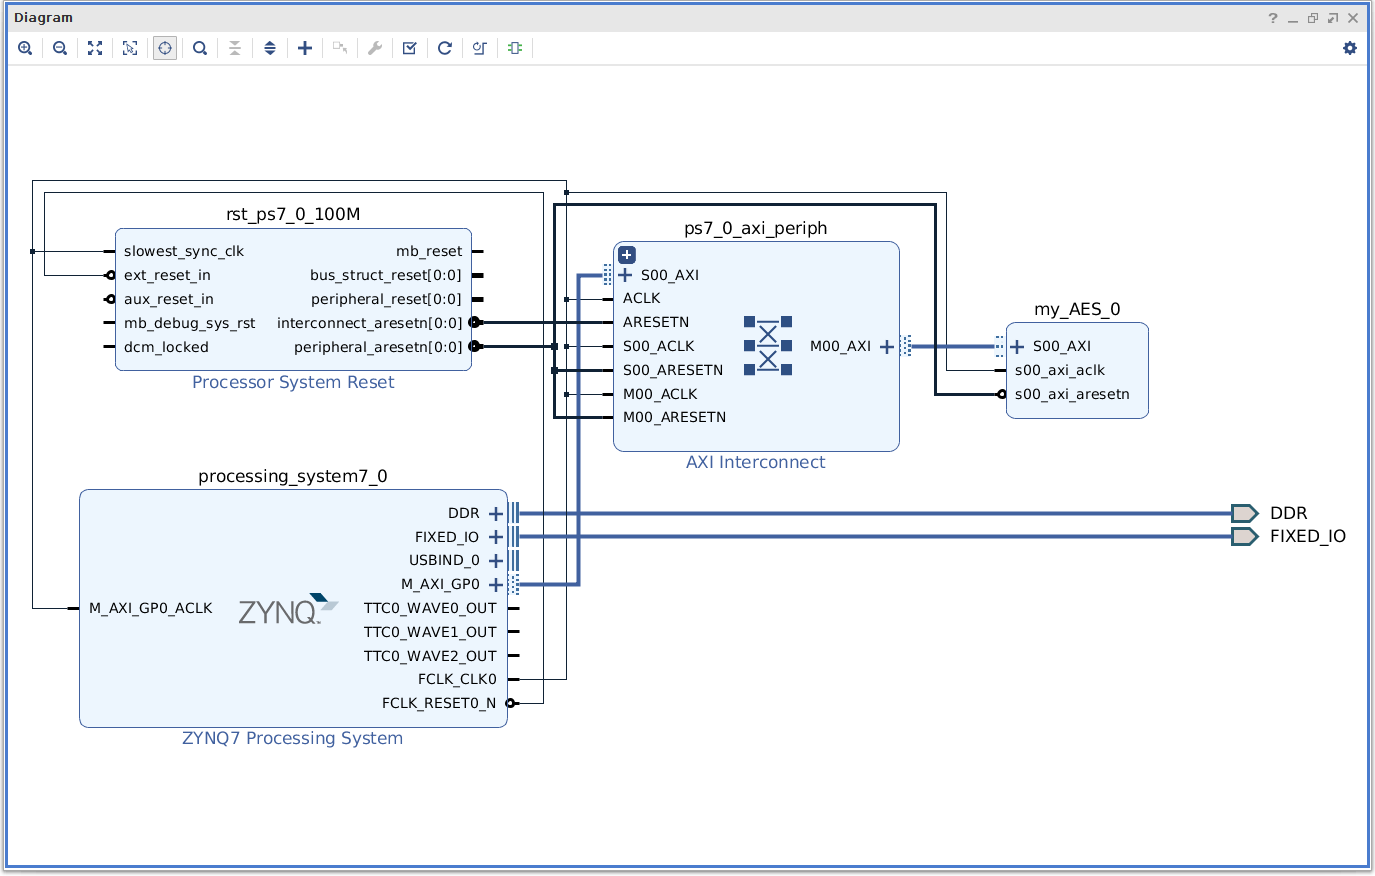
\includegraphics[scale=0.2]{vivado-tinyaes.png}
\end{figure}
\begin{verbatim}
\end{verbatim}
\end{frame}

%p20 兩個design 圖比較
\begin{frame}[fragile]
\frametitle{Uio Driver}
\begin{figure}
\centering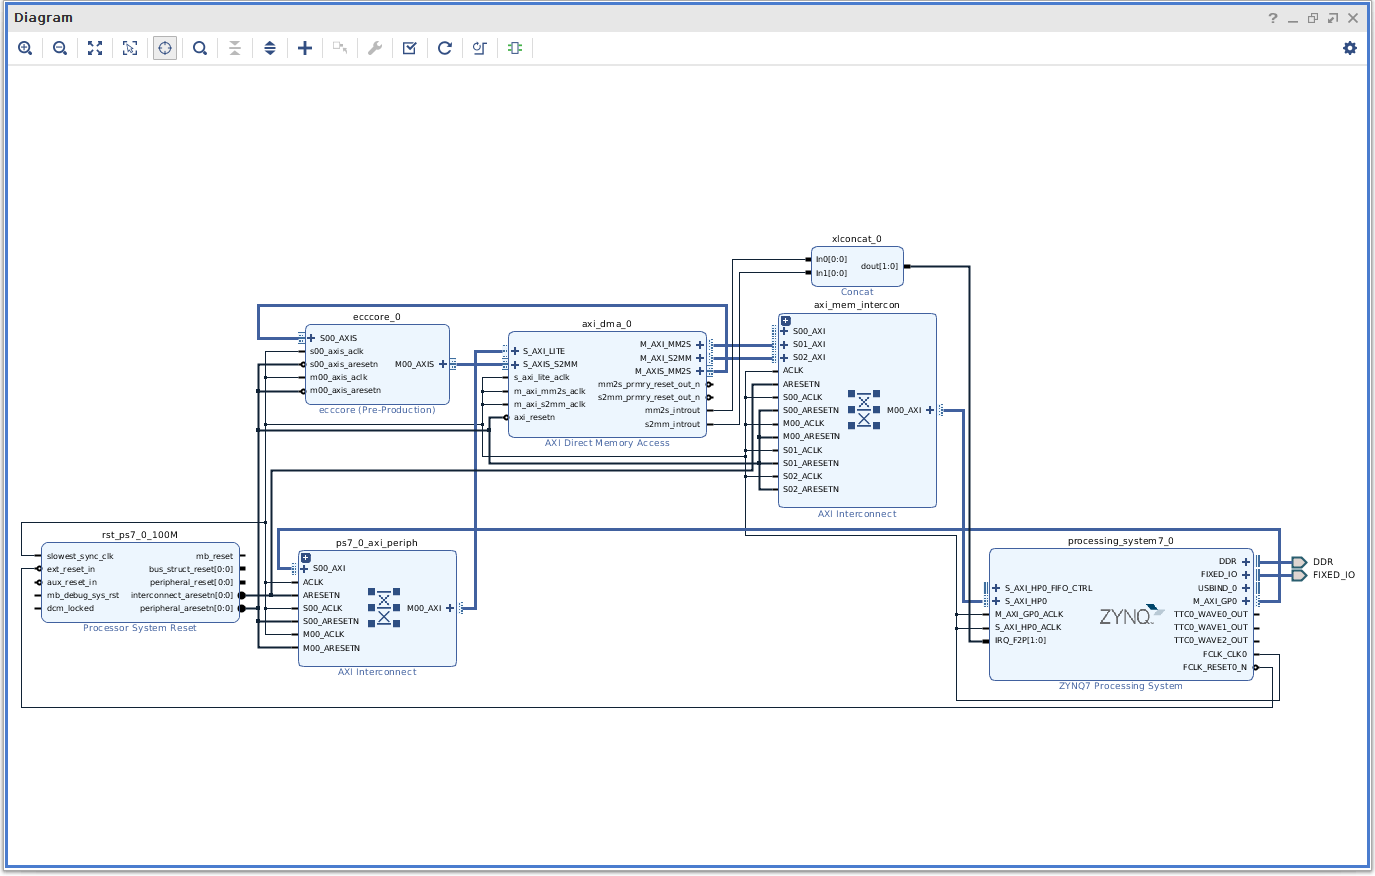
\includegraphics[scale=0.25]{vivado-ecc.png}
\end{figure}
\begin{verbatim}
\end{verbatim}
\end{frame}

%p21
\begin{frame}
%\frametitle{}
%\begin{itemize}
\centering DMA and AXI4
%\end{itemize}
\end{frame}

%p22
\begin{frame}
\frametitle{DMA and AXI4}
\centering DMA
\centering \\
\begin{itemize}
\item Direct memory access (DMA) is a feature of computer systems that allows certain hardware subsystems to access main system memory (Random-access memory), independent of the central processing unit (CPU).
\end{itemize}
\end{frame}

%p23
\begin{frame}
\frametitle{DMA and AXI4}
\centering AXI4
\centering \\
\begin{itemize}
\item AMBA® AXI4 (Advanced eXtensible Interface 4) is the fourth generation of the AMBA interface specification from ARM®. Xilinx Vivado Design Suite 2014 and ISE Design Suite 14 extends the Xilinx platform design methodology with the semiconductor industry's first AXI4 Compliant Plug-and-Play IP.
\end{itemize}
\end{frame}

%p24 ip register type
\begin{frame}[fragile]
\frametitle{DMA and AXI4}
\centering register type\\
\begin{figure}
\centering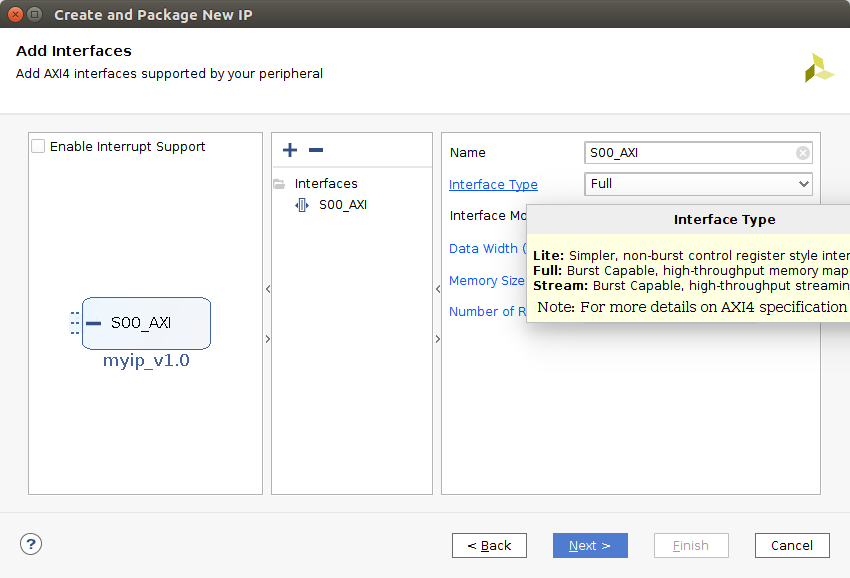
\includegraphics[scale=0.35]{register-type.png}
\end{figure}
\begin{verbatim}
\end{verbatim}
\end{frame}

%p25
\begin{frame}
\frametitle{DMA and AXI4}
\begin{itemize}
\item AXI4
	\begin{itemize}
	\item Traditional memory mapped address/data interface.
	\item Data burst support.
	\end{itemize}
\item AXI4-Lite
	\begin{itemize}
	\item Traditional memory mapped address/data interface.
	\item Single data cycle only.
	\end{itemize}
\item AXI4-stream
	\begin{itemize}
	\item Data-only burst.
	\end{itemize}
\end{itemize}
\end{frame}

%p26
\begin{frame}
\frametitle{DMA and AXI4}
\begin{figure}
\centering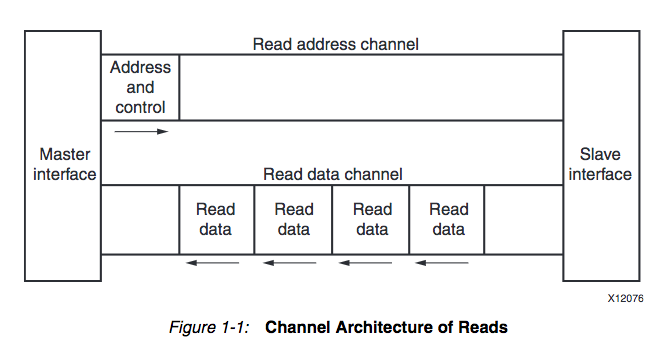
\includegraphics[scale=0.35]{axi-read.png}

\end{figure}
\end{frame}

%p27
\begin{frame}
\frametitle{DMA and AXI4}
\begin{figure}
\centering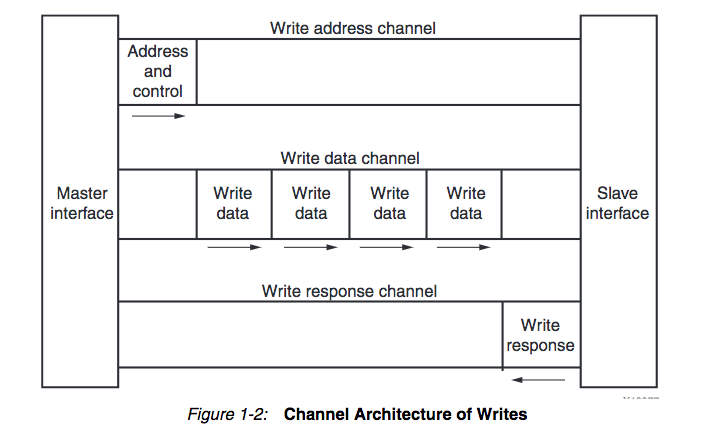
\includegraphics[scale=0.35]{axi-write.png}

\end{figure}
\end{frame}

%p27
\begin{frame}
\frametitle{DMA and AXI4}
\begin{figure}
\centering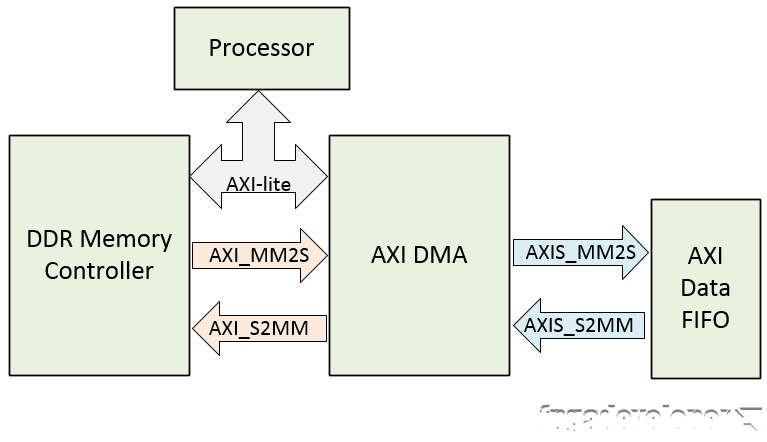
\includegraphics[scale=0.5]{axi-dma-example.png}
\end{figure}
\end{frame}



%p2
\begin{frame}
\frametitle{DMA and AXI4}

\begin{itemize}
\item If our custom IP uses AXI-Stream registers, we can't use UIO driver to mount our IP as a device.
\end{itemize}
\end{frame}

%p2
\begin{frame}
\frametitle{DMA and AXI4}
\centering But we still want to use our IP in userspace!\\
\pause
\centering\alert {->UIO driver modification}
\end{frame}

%p
\begin{frame}

\centering UIO driver modification
\end{frame}

%p2
\begin{frame}
\frametitle{UIO driver modification}
\centering In fact, DMA component is driven by the AXI-DMA module provided by xilinx linux kernel.\\
\centering So we can use Linux Kernel DMA API in our UIO driver.
\end{frame}

\begin{frame}
\frametitle{UIO driver modification}
\begin{itemize}
\item  DMA API\\
\begin{itemize}
\item   dma\_request\_slave\_channel\\
\item   dmaengine\_prep\_slave\_sg\\
\item   dmaengine\_submit
\end{itemize}
\end{itemize}

\end{frame}


%p2
\begin{frame}
\frametitle{UIO driver modification}
\centering We can create a virtual device node to apply UIO driver.
\end{frame}

%p8
\begin{frame}[fragile]
\frametitle{UIO driver modification}
\centering devicetree will be like:
\begin{figure}
\centering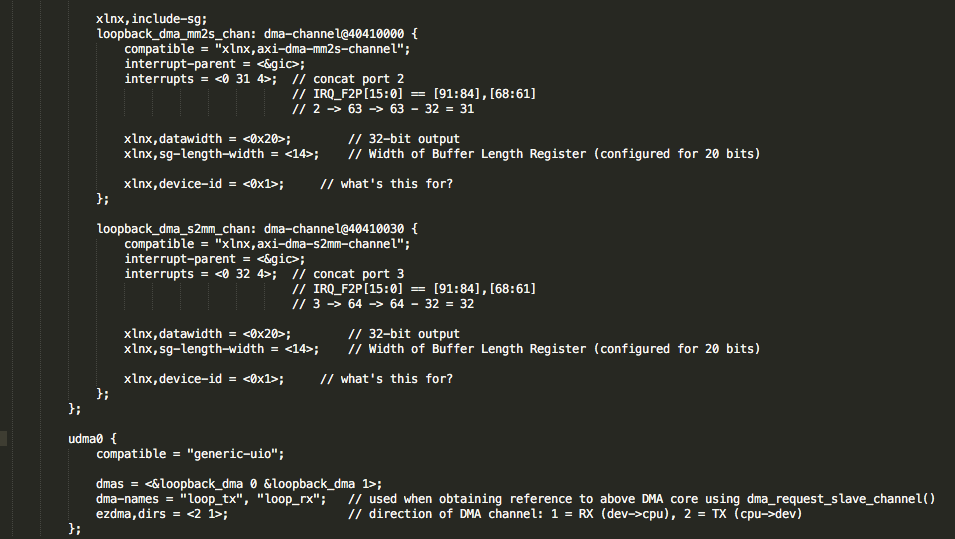
\includegraphics[scale=0.3]{devicetree2.png}
\end{figure}
\end{frame}


%p2
\begin{frame}[fragile]
\frametitle{UIO driver modification}
\centering recall\\
\begin{verbatim}
int fd = open("/dev/uio0", O_RDWR);

void *ptr = mmap(0, 0x10000, PROT_READ|PROT_WRITE, MAP_SHARED, fd, 0);

\end{verbatim}
\end{frame}

%p2
\begin{frame}
\frametitle{UIO driver modification}
read()
\centering \\
\begin{itemize}
\item Interrupts are handled by reading from /dev/uioX. A blocking read() from /dev/uioX will return as soon as an interrupt occurs. You can also use select() on /dev/uioX to wait for an interrupt. The integer value read from /dev/uioX represents the total interrupt count. You can use this number to figure out if you missed some interrupts.
\end{itemize}
\end{frame}

%p2
\begin{frame}
\frametitle{UIO driver modification}
write()
\centering \\
\begin{itemize}
\item UIO also implements a write() function,a write() to /dev/uioX will call the irqcontrol() function implemented by the driver.You have to write a 32-bit value that is usually either 0 or 1 to disable or enable interrupts. If a driver does not implement irqcontrol(), write() will return with -ENOSYS. 
\end{itemize}
\end{frame}


%p2
\begin{frame}
\frametitle{UIO driver modification}
\centering Virtual memory 
\centering \\
\begin{itemize}
\item The addresses a program may use to reference memory are distinguished from the addresses the memory system uses to identify physical storage sites, and program generated addresses are translated automatically to the corresponding machine addresses.
\end{itemize}
\end{frame}

%p
\begin{frame}[fragile]
\frametitle{UIO driver modification}
\begin{figure}
\centering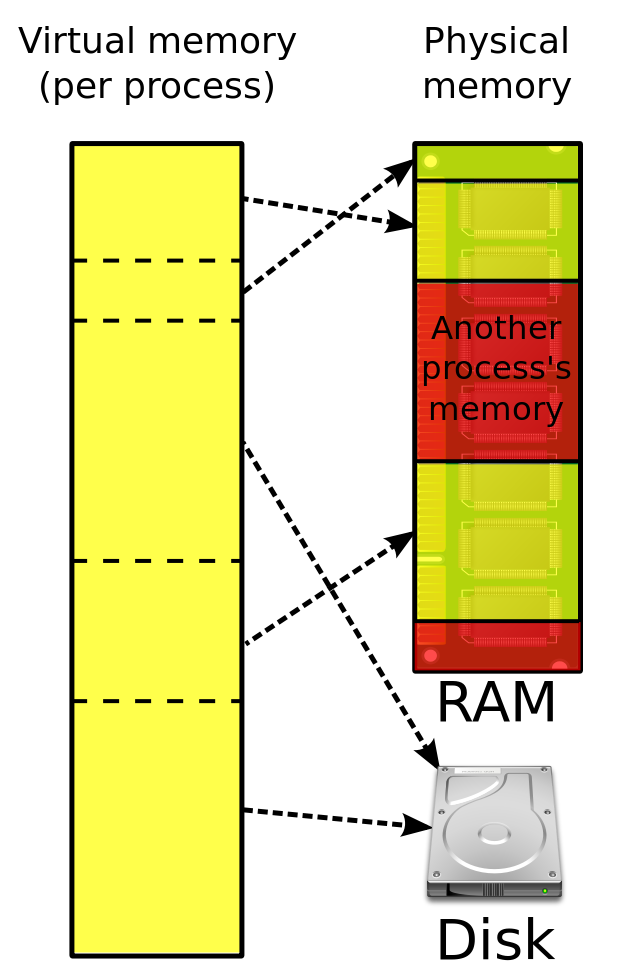
\includegraphics[scale=0.2]{virtual-memory.png}
\end{figure}
\end{frame}


%p2
\begin{frame}
\frametitle{UIO driver modification}
\centering Scatter-Gather\\

\centering Scatter-Gather DMA augments this technique by providing data transfers from one non-contiguous block of memory to another by means of a series of smaller contiguous-block transfers. The Lattice Scatter-Gather DMA Controller core implements a configurable, multi-channel, WISHBONE-compliant DMA controller with scatter-gather capability.

\end{frame}

%p2
\begin{frame}
\frametitle{UIO driver modification}
\centering Scatterlist\\
\begin{figure}
\centering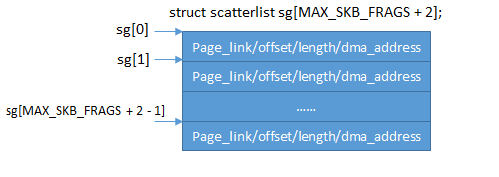
\includegraphics[scale=0.8]{scatterlist.png}
\end{figure}
\end{frame}


%p2
\begin{frame}
\centering Thanks!
\end{frame}

\end{document} 


